\newpage
\section{Approximating Functions with Other Functions}

\topic{January 26, 2022}
%
\begin{enumerate}
  \item Prove Series
\end{enumerate}

\begin{align}
  f(x) = \sum^M_{n = 0} a_n x^n \quad \text{Finite Power Series}
\end{align}

This is not the best way to approximate a function.

We choose the $a_n$'s so that the power series is ``close'' to $f(x)$ which
means we want to minimize the error.

We increase $M$ to get a better approximation.

The problem begins when you change $M$, the values of $a_n$'s change as well.
Therefore, recalculating is a lot of work.

If we let $M \to \infty$ and if $f \in C^\infty$, so then
$a_n = \frac{f^{(n)}(0)}{n!}$ and we get the Taylor series.

\note $C^\infty$: C means Continuous and the $\infty$ indicates the number of
derivatives that are continuous.

Problem: This is only good inside the radius of convergence.
%
\bigbreak
%
A Fourier Series is a trigonometric polynomial
%
\begin{align}
  \sum_{n = 0}^M a_n \FS + b_n \FC \longleftarrow \text{period = } 2L
\end{align}

We use Fourier Series for a function on a bounded interval and we will use $x\in [-L, L]$

\subsection{Advantages of Fourier Series}

\begin{enumerate}
  \item If $M$ increases, we only need to calculate the new $a_n$'s and
  $b_n$'s. This property is due to the fact that the basis functions are
  orthogonal.

  \item If $M = \infty$ and $f$ is continuous, then the Fourier Series $=
  f(x) \forall x \in (-L, L)$. Our interval must be open for the case that
  $f(-L) \neq f(L)$.
\end{enumerate}

Basis Functions : $\FS, \FC$
%
\begin{center}
  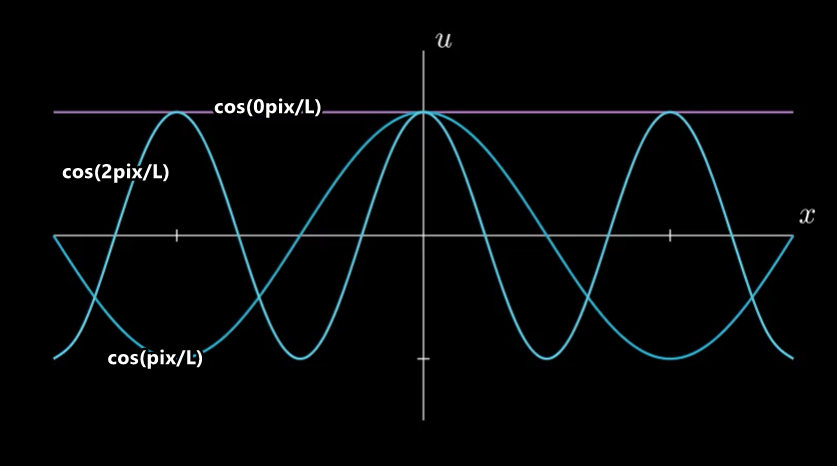
\includegraphics[height=5cm]{Fourier Basis Functions}
\end{center}

What happens if you use a Fourier Series on a discontinuous function?
%
\begin{align}
  f(x) & =
  \begin{cases}
    1 & x \in (-4, 6)\\
    0 & x \in [-10, -4] \bigcup [6, 10]
  \end{cases}
\end{align}

\begin{center}
  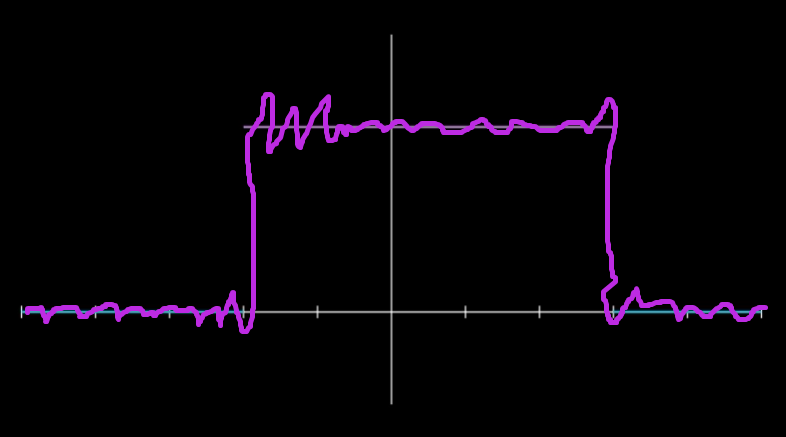
\includegraphics[height=5cm]{Fourier Finite Fourier Series}
\end{center}

The Oscillations around the discontinuities are called Gibbs phenomenon. As
$M$ increases, the oscillation's amplitude does not change. However, the
oscillations do get progressively closer to the discontinuities.

\begin{center}
  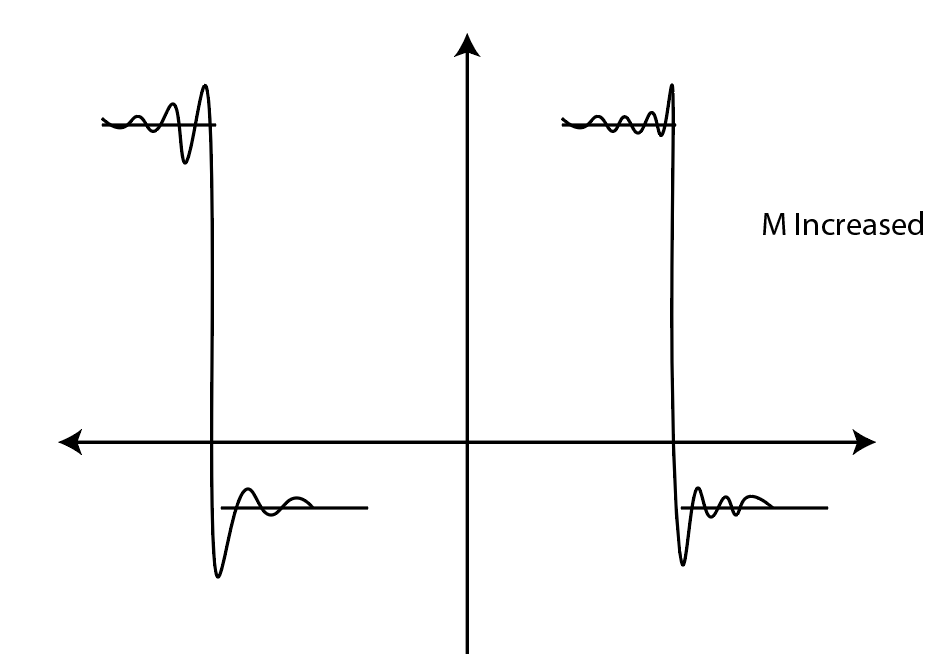
\includegraphics[height=5cm]{Fourier M}
\end{center}

If $M = \infty$, then we have:
%
\begin{align}
  \text{Fourier Series } =
  \begin{cases}
    f(x) & = \text{ if $x$ is a point of continuity }\\
    \lim_{c \to 0^+} \frac{f(x + c) + f(x - c)}{2}
    & \text{ if x is a point of discontinuity}
  \end{cases}
\end{align}

\begin{center}
  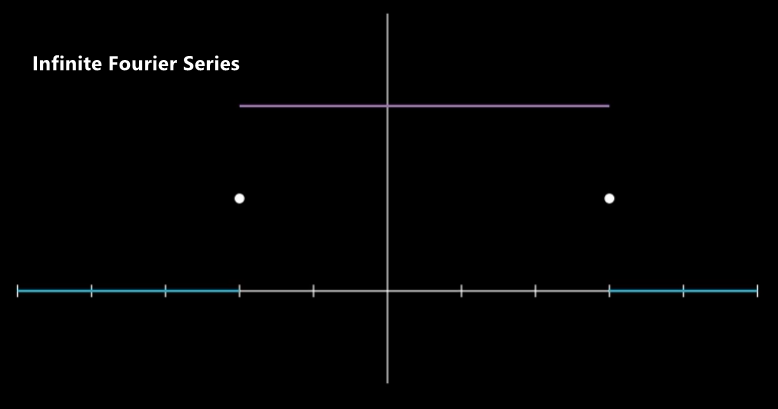
\includegraphics[height=5cm]{Fourier Infinite Fourier Series}
\end{center}

\subsection{Orthogonality}

Recall: The vectors
\begin{align}
  u =
  \begin{bmatrix}
    u_1\\
    u_2\\
    \vdots\\
    u_n
  \end{bmatrix}
  \qquad \text{and} \qquad
  v =
  \begin{bmatrix}
    v_1\\
    v_2\\
    \vdots\\
    v_n
  \end{bmatrix}
\end{align}

are orthogonal if the dot product is zero.

\begin{align}
  u \circ v & = \sum^n_{i = 1} u_i v_i = 0
\end{align}

We want to generalize this to function $x \in [-L, L]$.

\dfn Two functions $f(x)$ and $g(x)$ are orthogonal on $[a, b]$ if

\begin{align}
  \int^b_a f(x)g(x) \dx & = 0
\end{align}

% Note, minimal notes were taken, refer to Numerical Analysis notes
\subsection{Fourier Series}

\thm All basis functions in the Fourier Series are mutually orthogonal

\begin{align}
  \int^L_{-L} \sin\Big(\frac{m \pi x}{L}\Big) \FS \dx & = 0 \quad n \neq m\\
  \int^L_{-L} \cos\Big(\frac{m \pi x}{L}\Big) \FC \dx & = 0 \quad n \neq m
\end{align}
What happens if $m = n$?
\begin{align}
  \int^L_{-L} \sin^2\Big( \frac{m \pi x}{L} \Big) \dx
\end{align}

Here, we want to use the double angle formula:
$\cos(2\theta) = 1 - 2\sin^2 \theta$.
%
\begin{align}
  \int^L_{-L} \sin^2\Big( \frac{m \pi x}{L} \Big) \dx & =
  \frac{1}{2} \int^L_{-L} 1 - \cos\Big(\frac{2 m \pi x}{L}\Big) \dx\\ & =
  \frac{1}{2} \Big[ x - \frac{L}{2 m \pi}
  \sin\Big(\frac{2 m \pi x}{L}\Big)\Big]^L_{-L}\\ & =
  \frac{1}{2} \Big[L - \frac{L}{2 m \pi}
  \sin(2 m \pi) - \Big(-L - \frac{2}{2 m \pi} \sin(-2 m \pi)\Big)\Big]\\ & =
  L
\end{align}

\topic{January 28, 2022}

Similarly,
%
\begin{align}
  \int^L_{-L} \cos^2 (\frac{n\pi x}{L}) \dx & = L
\end{align}

If $n = 0$,
%
\begin{align}
  \int^L_{-L} 1 \dx & = 2L
\end{align}

\note You cannot differentiate the Fourier Series term-by-term $f'(x)$ like
you can with Taylor series.

Let's show $\cos(\frac{n \pi x}{L})$ and $\sin(\frac{m \pi x}{L})$ are
orthogonal on $[-L, L]$.
%
\begin{align}
  \int^L_{-L} \sin\Big(\frac{m \pi x}{L}\Big) \FC \dx
  & = \frac{1}{2} \int^L_{-L}
  \sin\Big( \frac{(m + n) \pi x}{L} \Big)
  + \sin\Big( \frac{(m - n) \pi x}{L} \Big) \dx\\
  & = - \frac{1}{2} \Big[ \frac{L}{(m + n) \pi}
  \cos\Big(\frac{(m + n) \pi x}{L} \Big)
  + \frac{L}{(m - n)\pi} \cos\Big( \frac{(m - n) \pi x}{L} \Big) \Big]^L_{-L}
\end{align}

Here, we expand our difference and notice we have even and odd functions.

In general, the coefficients are:
%
\begin{align}
  a_n & = \frac{1}{L} \int^L_{-L} f(x) \FS \dx\\
  b_n & = \frac{1}{L} \int^L_{-L} f(x) \FC \dx\\
  b_0 & = \frac{1}{2L} \int^L_{-L} f(x) \dx
\end{align}

\Ex $f(x) = x, \quad x \in [-3, 3]$.

Find the Fourier Series for $f$.
%
\begin{align}
  a_n & = \frac{1}{3} \int^3_{-3} x \FS \dx
\end{align}

Here, we want to integrate by parts:
%
\begin{center}
  \begin{tabular}{c|c}
    $x$ & $\FS$\\
    \hline
    $1$ & $- \frac{3}{n \pi} \FC$\\
    \hline
    $0$ & $- \frac{9}{n^2 \pi^2} \FS$
  \end{tabular}
  \note $L = 3$.
\end{center}

\begin{align}
  & = \frac{1}{3} \Big[ -\frac{3 x}{n \pi}
  \cos\Big( \frac{n \pi x}{3} \Big) \Big]^3_{-3}
  + \Big[ \Big( \frac{3}{n \pi} \Big)^2
  \sin\Big( \frac{n \pi x}{3} \Big)\Big]^3_{-3}\\
  & = \frac{1}{3} \Bigg[ -\frac{9}{n \pi} \cos(n \pi) + \frac{9}{n^2 \pi^2}
  \sin(n \pi) -
  \Big( +\frac{9}{n \pi} \cos(-n \pi)
  + \frac{9}{n^2 \pi^2} \sin(-n \pi) \Big)\Bigg]\\
  & = -\frac{6}{n \pi} \cos(n \pi)
\end{align}

The Fourier Series is not valid at $x = \pm 3$ since it is not continuous at $\pm 3$.

Let's say $f(x)$ is odd, then $\displaystyle f(x) = \sum^\infty_{n = 1} a_n \FS$

Let's say $f(x)$ is even, then $\displaystyle f(x) = \sum^\infty_{n = 1} b_n \FC$

If we are only interested in the behavior of $f(x)$ on $[0, L$, then we can either use a Fourier Sine Series $\displaystyle f(x) = \sum^\infty_{n = 1} a_n \FS$ or a Fourier series $f(x) = \sum^\infty_{n = 0} b_n \FC$.
